
\section{Introduction}

Time series forecasting (TSF) plays a key role in data-driven decision-making across critical domains, including financial market analysis~\cite{sako2022neural}, energy demand planning~\cite{kotzur2018time}, and traffic flow management~\cite{li2015trend}. Over the years, a spectrum of approaches—from classical statistical models to machine learning and deep learning—has been developed to improve forecasting accuracy.

Classical statistical methods such as ARIMA \citep{zhang2003time}, ETS \citep{hyndman2008forecasting}, and Theta \citep{assimakopoulos2000theta} have long been used to predict future data by leveraging the statistical properties of single samples. Machine learning methods such as XGBoost\citep{chen2016xgboost} and LightGBM\citep{ke2017lightgbm} remain highly effective due to their interpretability and ability to model nonlinear relationships. Recent advancements in deep learning techniques have made them particularly effective at modeling complex temporal dependencies and non-stationary data in time series forecasting. Methodological analysis covers pioneering architectures such as sequence dependency modeling of RNNs \citep{hewamalage2021recurrent,salinas2020deepar}, TCNs \citep{hewage2020temporal} and transformer-based models \citep{ijcai2023p759}, which improve generalization through shared representations across multiple time series.

\begin{figure*}[t] 
    \centering
    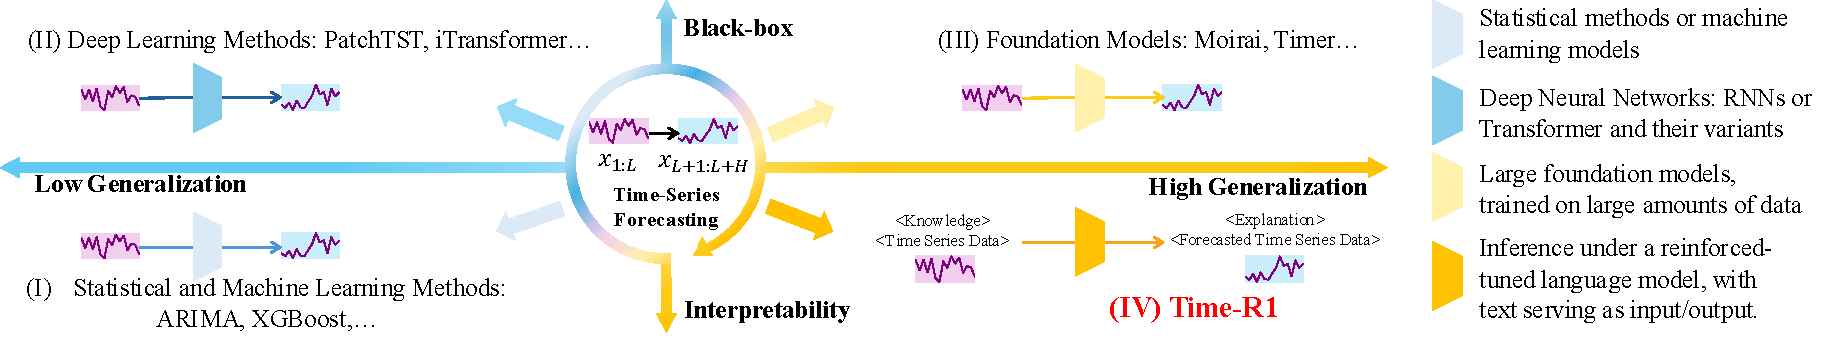
\includegraphics[width=1\textwidth]{images/7_comparison_.pdf} 
    \vspace{-0.1in}
    \caption{A taxonomy of TSF paradigms from statistical/ML models to deep learning and foundation models, organized by increasing generalization and model transparency. \Ours represents a reasoning-oriented paradigm that leverages time-series knowledge and explanation generation to support forecasting.} 
    \vspace{-0.16in}
    \label{fig:7_comparison} 
    \vspace{-0.04in}
\end{figure*}

Although the specific techniques vary, most existing TSF methods follow a similar "fast thinking" paradigm~\citep{wang2024tabletime,wang2025can,liu2025evaluating}. Specifically focusing on single-step prediction accuracy, these methods typically employ sequential models to encode historical values and use one-step decoding to directly map past observations to future values. Although effective in benchmarks, their underlying logic is largely based on pattern recognition and trend prediction, lacking an explicit reasoning process. However, in real-world scenarios, time series often reflect more complex temporal logic, which should not merely be 'fitted'—they should be understood and reasoned.


To address this issue, a growing body of work explores how large language models (LLMs) can support time series forecasting. Specifically, recent methods use LLMs to analyze temporal dynamics and learn informative representations, which in turn improve TSF models \citep{chang2023llm4ts,liu2025calf,jin2023time}. These approaches leverage LLMs to incorporate contextual information, such as textual metadata \citep{gruver2023large}. This additional context often improves cross-domain generalization \citep{liu2024time, dooley2023forecastpfn} and enables explanations that support forecasting decisions \citep{tan2024language}.


However, despite their potential, current LLM-based TSF methods face three key limitations:
\textit{First}, a partial misalignment of time series domain knowledge, and limited reasoning capabilities. General linguistic knowledge in LLMs often mismatches the temporal patterns and causal mechanisms required for time series tasks, leading to suboptimal performance \citep{zhou2023one}.
\textit{Second}, a lack of generalization from experiential learning. While effective in fitting historical patterns, they struggle with understanding dynamics or adapting to new, unseen scenarios, which limits their out-of-distribution performance.
\textit{Third}, absence of progressive reasoning. These models map history to future directly without detecting regime changes or performing step-by-step inference, resembling fast (not deliberate) thinking for time series.
These issues lead to a central question: \textbf{Can we improve time series forecasting performance by training LLMs to acquire time series reasoning capabilities?} 

Motivated by this question, we propose \Ours, a novel LLM-based time series forecasting framework that trains large language models to acquire slow-thinking reasoning capabilities for future-trend forecasting. 
% At its core, \Ours leverages LLMs as the time series reasoning backbone and introduces a two-stage reinforcement fine-tuning (RFT) optimization framework:
\Ours adopts an LLM as the reasoning backbone and follows a curriculum-style RFT optimization: it first warm-starts reasoning and formatting with synthetic step-by-step temporal analyses, and then progressively improves generalization through reward-driven policy optimization.
\textit{First}, we begin with warm-up supervised fine-tuning. The model is fine-tuned for supervised pattern alignment, learning both effective reasoning patterns and accurate output formatting using synthetic reasoning trajectories that demonstrate step-by-step temporal analysis. \textit{Second}, the model is refined through reinforcement learning for generalization, using fine-grained, multi-objective rewards specifically designed for forecasting tasks, improving temporal coherence and multi-horizon accuracy. Notably, we propose GRIP (group-based relative importance for policy optimization), which optimizes LLM reasoning paths in TSF through a non-uniform sampling strategy and adaptive weighting. Extensive experiments are conducted on real-world datasets, showing that \Ours effectively enhances forecast performance through the slow thinking paradigm. Our main contributions are as follows:

\begin{itemize}[leftmargin=10pt, itemsep=1pt]
  % \setlength{\itemsep}{1pt} 
  % \setlength{\parskip}{2pt} 
  \item We introduce time series reasoning by training LLMs to adopt a slow-thinking paradigm that reasons explicitly over the temporal patterns for final forecasting.
  \item We design a RFT framework that enhances the reasoning ability of LLMs. We introduce a fine-grained reward specifically for TSF, along with a novel sampling strategy for RL optimization.
  \item Extensive experiments demonstrate the effectiveness of \Ours, showing that it enhances LLM reasoning and further improves generalization and explainability via deliberate slow thinking.
\end{itemize}

